\subsection{Caso testigo}
\label{caso-testigo}

Habiendo desarrollado la propuesta de rediseño que motiva el presente trabajo, creemos conveniente tomar un caso testigo que sirva de ejemplo práctico para hacer concretos los conceptos teóricos que hemos tenido en cuenta para el análisis, a la vez que sirva de disparador para una implementación preliminar acotada del nuevo diseño sobre los elementos de la nube de servicios.

\subsubsection{Alcance}

La situación que utilizaremos como caso testigo es el proceso de registro de un nuevo usuario de \gls{acro:sso} de la nube de servicios de la \unlp. Si bien \textit{a priori} puede parecer un tanto sencillo para tomarlo de referencia, una vez que definamos concretamente todos los pasos involucrados en este proceso se hará evidente la elección realizada.

Aquellos agentes que forman parte del personal de la UNLP pueden tener un usuario único para acceder a las aplicaciones que nuestra Dirección desarrolla, ya sea para consultar sus recibos de haberes, utilizar una aplicación como parte de sus tareas diarias, presentar proyectos de extensión cuando la convocatoria se encuentre abierta o para acceder a cualquier aplicación que a futuro pudiéramos publicar. Para registrar su usuario, el agente dispone de dos vías:

\begin{itemize}
  \item La vía analógica: solicitando la creación del usuario, de manera presencial y por escrito, a la oficina de Personal de alguna de las Dependencias donde desempeña sus funciones. Por tratarse de un proceso manual y \eng{offline}, no lo consideraremos para este caso testigo.
  \item La vía digital: utilizando la \hyperref[anexo:detalle-clientes:sso]{aplicación de autogestión} que hemos desarrollado para realizar el registro del nuevo usuario en línea. \textit{Esta} es la vía que utilizaremos en nuestro planteo.
\end{itemize}

En el proceso de autogestión de un nuevo usuario, el agente debe completar los datos solicitados en una serie de pasos preestablecidos que lo guían hasta llegar a obtener el acceso a las aplicaciones que utilizan este esquema de \gls{acro:sso}\footnote{En realidad, inicialmente obtiene acceso únicamente a ver sus \hyperref[anexo:detalle-clientes:recibos]{recibos de haberes} y cargar su \textit{currículum de extensionista} en la aplicación de \hyperref[anexo:detalle-clientes:extension]{Proyectos de Extensión}. Para ingresar al resto de las aplicaciones un usuario autorizado le debe asignar los roles necesarios para cada aplicación.}. Podemos resumir estos pasos para el registro en:

\begin{enumerate}
  \item El agente ingresa a la aplicación de autogestión e indica que desea registrar un nuevo usuario.

  \item La aplicación le solicita que se identifique mediante su documento de identidad.

  \item Una vez identificado el usuario, se le pide que indique en qué Dependencias de la UNLP presta servicios a modo de \gls{term:captcha} para evitar bots que intenten registrar usuarios en masa y personas malintencionadas que deseen registrar usuarios en nombre de agentes reales.

  \item Al validar correctamente esta información, se pide al agente que elija un nombre de usuario que utilizará como identificación y algunos datos más para contactarlo en caso de tener problemas con su dirección de correo electrónico principal.

  \item Finalmente, se le presentan todos los datos ingresados para su confirmación y si el agente los acepta, se le envía un correo electrónico con un formulario para presentar firmado en la oficina de Personal de alguna de las Dependencias donde presta servicios, teniendo un paso de validación humana de la información\footnote{Este paso adicional, si bien puede sonar contradictorio con el resto del proceso \eng{online} planteado, fue requerido por las autoridades de la Universidad para fortalecer los chequeos realizados sobre los datos recibidos mediante este servicio público de registro.}.

  \item Luego de presentar ese formulario y que sus datos sean debidamente corroborados por algún empleado de la oficina de Personal correspondiente, el usuario es aprobado y se dispara el envío de un nuevo correo al agente, en el cual se le consignan su usuario y una clave provisoria para que ingrese por primera vez a los sistemas de la UNLP. Con este paso, se finaliza el proceso de registro del nuevo usuario para el agente.
\end{enumerate}

Desde el punto de vista de nuestra aplicación, este proceso se ve un tanto reducido ya que no es necesario que incluyamos los pasos que ocurren por fuera del \textit{mundo virtual} o en la aplicación de gestión que utilizan los empleados de las oficinas de Personal de las Dependencias, ya que quedan afuera de su alcance. Formalizaremos los pasos que se realizan en este sistema con el diagrama de flujos presentado a continuación para su mayor referencia.

\begin{figure}[H]
  \centering
  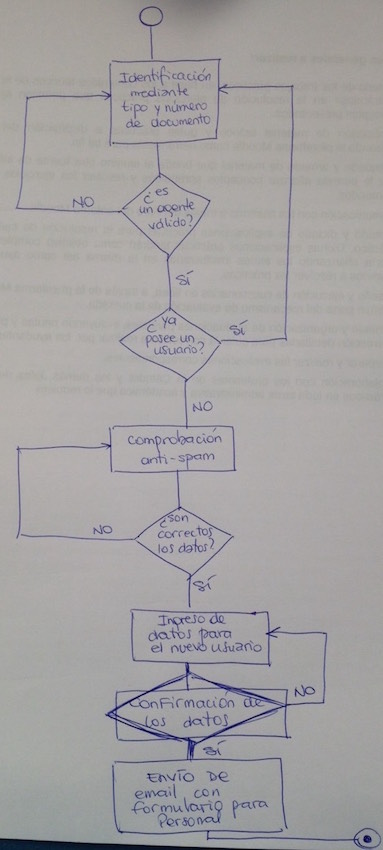
\includegraphics[width=\textwidth,height=0.5\textheight,keepaspectratio]{src/images/05-capitulo-5/diagrama-flujo-registro.jpg}
  \caption{Proceso de autoregistro de un nuevo usuario de acceso único}
  \label{fig:diagrama-flujo-registro}
\end{figure}

Realizando una descomposición en servicios del proceso anterior, identificamos las siguientes dependencias con servicios de la nueva nube\todo{¿Dar un nombre a la nueva nube? - @ncuesta}:

\begin{itemize}
  \item \textbf{Servicios de referencia:} para visualizar y marcar las Dependencias (o Unidades Académicas) y para ofrecer para su selección los tipos de documento de identidad.
  \item \textbf{Servicios de información sobre el personal:} como vía para identificar a la persona y luego consultar las Unidades Académicas en las cuales presta sus servicios.
  \item \textbf{Servicios de usuarios:} para la consulta de la existencia de un usuario para la persona seleccionada y para la creación del nuevo usuario.
  \item \textbf{Servicio de notificaciones:} para el envío de correos electrónicos.\todo{Ver si lo incluimos}
\end{itemize}

El desarrollo del prototipo funcional implica, además de realizar el \gls{term:refactor} de la aplicación cliente de registro existente en la actualidad, la implementación desde cero de los servicios (y la lógica en el cliente para el acceso a éstos) siguiendo la nueva estructura, el protocolo de autenticación y los estándares para la comunicación de nuestra propuesta. Al hacer esta prueba de concepto, hemos obtenido \todo{¿Está bien usar el pasado acá?} una noción palpable del costo de llevar estos cambios a nuestras aplicaciones, lo cual da un alto valor agregado a esta experiencia cuando llegue el momento de estimar el tiempo y los recursos necesarios para llevar adelante este cambio en los desarrollos existentes y futuros de nuestro equipo.

Hemos elegido este caso testigo porque se compone de una serie de interacciones entre distintos servicios que brindan una noción de la complejidad que pueden tener las operaciones a realizar utilizando la nube de servicios, más allá de las simples consultas de datos de referencia que habitualmente manejamos. El hecho de incorporar diferentes servicios, englobados en distintas áreas de acción, nos permite también mostrar cómo funcionan las instancias de las aplicaciones que proveen esos servicios, cómo interactúan con la aplicación cliente y con los elementos intermediarios de la comunicación (entiéndase \eng{caches} compartidas, balanceadores de carga, \eng{proxies} reversos y la capa de mediación ofrecida por \nameref{soa:tecnologias:kong}).

En este informe intentaremos no entrar en detalles innecesarios sobre la implementación de la aplicación cliente ni de la capa de lógica del negocio de los servicios, para sí ahondar sobre temas relevantes desde el punto de vista de la comprensión de las entidades participantes en las comunicaciones. De todas formas, se deja disponible el código fuente de los distintos apartados para su referencia en \todo{Agregar link al código fuente de la implementación}.


\subsubsection{Desarrollo de un prototipo funcional}

Documentar el desarrollo
